\section{Background}
\label{sec:Background}

\subsection{Python}

Python~\cite{Python} is a high-productivity programming language used in a
wide variety of domains such as web services, program steering, data analysis,
and conventional scripting. It is also widely used for artificial
intelligence, game engines, and scientific computing~\cite{SciPy}. Python's
concise syntax combined with dynamic typing, built-in data structures, and a
rich standard library facilitates rapid program implementation. The language
implementation is also very portable across a variety of processor
architectures and operating systems. However, Python's rich semantics and
interpreted execution incurs run-time overhead. This penalty is often offset
by savings in development time and the use of high-performance C libraries
such as NumPy~\cite{NumPy:2007}. We use Python both for prototyping and
application development.

An import aspect of Python data types is that almost all of them can be easily serialized with the {\it pickle} module.  This module creates a byte stream of a Python object instance which can be {\it unpickled} at a later time.

\subsection{Stackless Python}
\label{sec:StacklessPython}

The standard Python implementation, written in C, is referred to as {\it
CPython}. This implementation executes Python programs by first
compiling all source files into Python bytecode. The bytecode is then
interpreted by the Python run-time system. To support function calls and
method invocation, the run-time system uses the C stack to recursively
call the main interpreter loop. This means that as Python programs
run, their execution state consists of high-level Python object
instances and C activation records. This tight coupling of
architecture-specific state and language objects makes it difficult to
capture the state of a Python program.

Stackless Python~\cite{Stackless:2007, Tismer:2000:StacklessPython} is a modified implementation of CPython that solves the state capture problem by decoupling the C stack from the Python execution stack.  A significant result of this modification is that the execution state of a Python program can be pickled to a byte stream.  This functionality serves as the basis for our distributed state management mechanism.  In addition to decoupling the C stack, Stackless Python also adds language support for cooperative {\it tasklets} and communication between tasklets using {\it channels}.  These features make it possible to support thousands of cooperative execution streams in a single Python instance.

\subsection{River}
\label{sec:River}

River is a Python-based framework for distributed
computing~\cite{River:2007}. River consists of a set of Python classes
that provide a core interface and the underlying run-time system. A
River program consists of one or more {\it virtual resources} (VRs)
that execute on River virtual machines (VMs); see
Figure~\ref{fig:core-execution}. VMs can exist locally or remotely and
VRs are named using UUIDs~\cite{RFC4122}. A VM is simply a Python
interpreter running the River run-time system. An initiating VR can
discover existing VMs and deploy itself or other VRs onto selected VMs.
Once running, VRs communicate with each other using a mechanism called
{\it super flexible messaging} (SFM) for sending and receiving
dynamically typed packets~\cite{Fedosov:2007:SFM}.  SFM makes it easy to send arbitrary data as attribute-value pairs and
selectively receive messages based on matching attribute names and subsets of
attribute values. 
%This powerful mechanism eliminates the need to define a fixed packet structure or specify fixed remote interfaces.  
See Listing~\ref{ex:simple-program} for a minimal River program that discovers available VMs then starts VRs on these VMs.  Each child VR sends a message back to the initiating VR.

\begin{figure}[htb]
\centering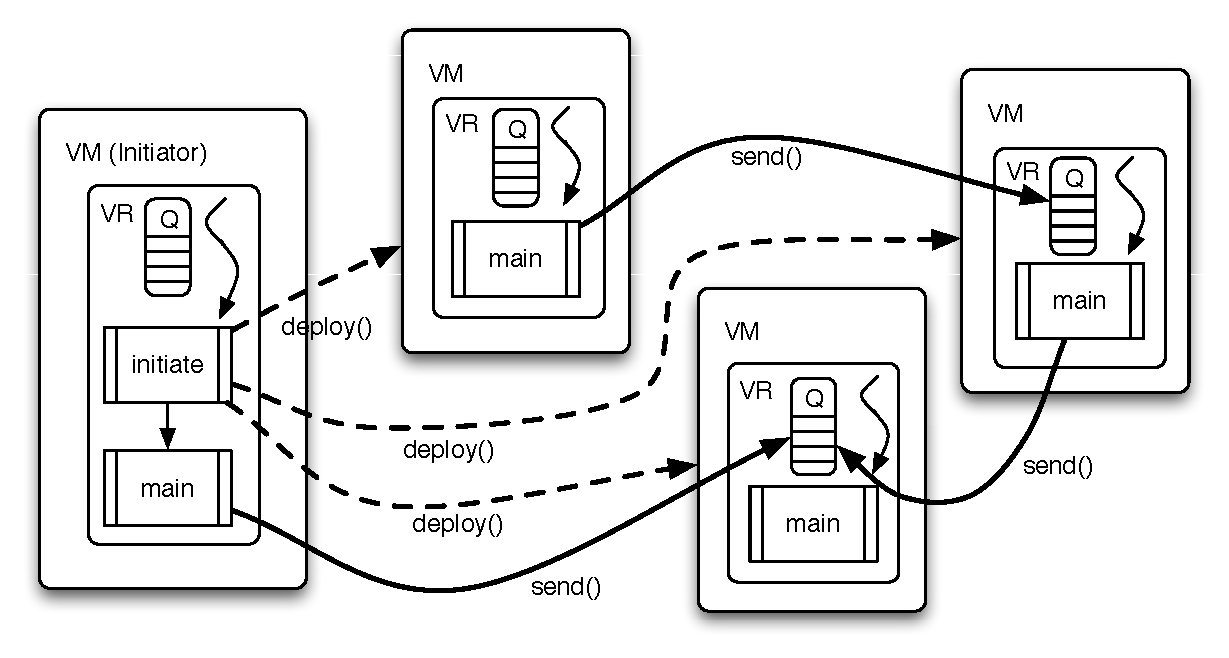
\epsfig{file=core-execution.eps,width=3.3in}
\caption{The Core River Abstractions}\label{fig:core-execution}
\end{figure}


%\begin{figure}[htb]
\begin{listing}
\scriptsize
\begin{verbatim}


from socket import gethostname
from river.core.vr import VR

class Hello(VR):
  def initiate(self):
    discovered = self.discover()
    allocated = self.allocate(discovered)
    deployed = self.deploy(allocated, 
                           module=self.__module__)
    self.vrlist = [vm.uuid for vm in deployed]
    return True

  def main(self):
    if self.parent is None:
      for vr in self.vrlist:
        msg = self.recv(src=vr)
        print '%s says hello' % msg.myname
    else:
      self.send(dest=self.parent, myname=gethostname())
\end{verbatim}
\normalsize
\caption{A Simple River Program}
\label{ex:simple-program}
\end{listing}
%\end{figure}

River was originally conceived with fault-tolerance in mind.  The Core API and underlying programming model supports execution transparency through ``soft'' names via UUIDs and decoupled message queues.  The rest of this paper describes the checkpointing and migration mechanism we have implemented in River.
